\section{FFT}
\subsection{DFT}
\(\operatorname{DFS}[\tilde{x}[n]]=\widetilde{X}[k]=\sum_{n=0}^{N-1} \tilde{x}[n] W^{n k}\)
\(\operatorname{IDFS}[\widetilde{X}[k]]=\tilde{x}[n]=\frac{1}{N} \sum_{k=0}^{N-1} \widetilde{X}[k] W^{-n k}\)

\(\displaystyle \operatorname{DFT}[x[n]]=X[k]=\sum_{n=0}^{N -1} x[n] W^{n k}, 0 \leq  k \leq  N-1\)
\(\displaystyle \operatorname{IDFT}[X[k]]=x[n]=\frac{1}{N} \sum_{k=0}^{N-1} X[k] W^{-n k}\)
\(W_N=W=e^{-j\,\frac{2\pi}{N}}\)

矩阵序列:\(R_N[n]=1,n\in [0,N-1]\)

\textbf{数据采样参数}\\
采样时间间隔:\(T_s=\frac{1}{f_s}<\frac{1}{2f_{\max}}\)\\
采样总时间:频率分辨率\(f_1\),\(T_1\geq\frac{1}{f_1}\)\\
采样数据点:\(N=\frac{T_1}{T_s}\),向上取到\(2^n\)\\

\vspace{-10pt}
\begin{figure}[H]
    \centering
    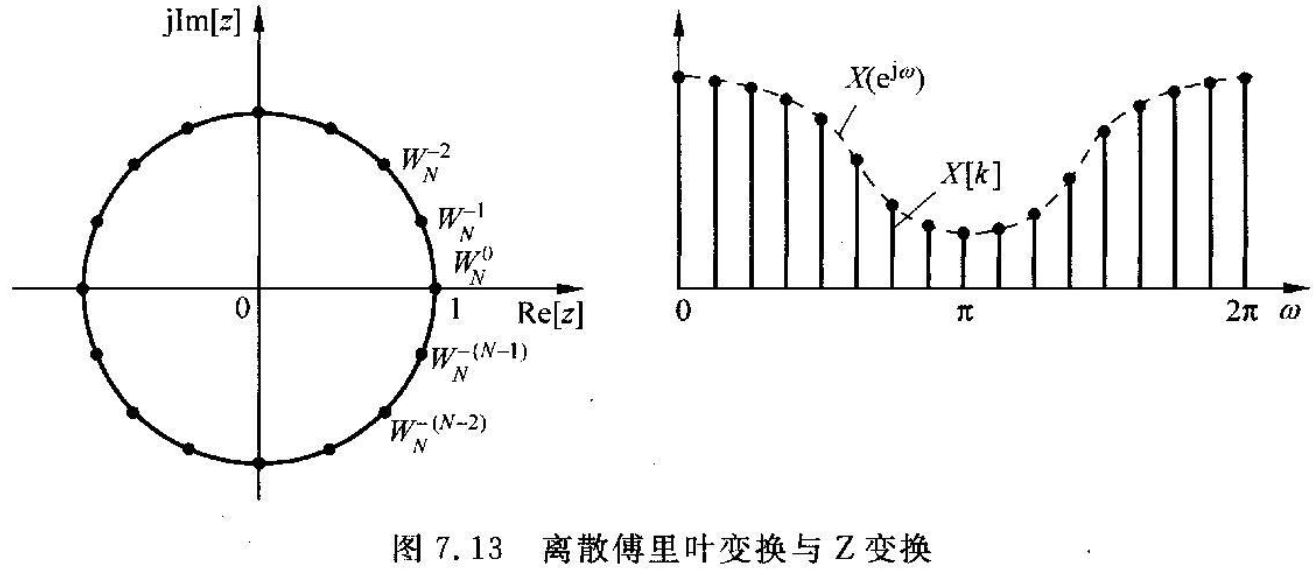
\includegraphics[width=\linewidth]{figure/Pasted image 20220611024619.png}
\end{figure}
\vspace{-10pt}

\subsection{圆卷积}
$x[n] (N) y[n] =\sum_{m=0}^{N-1} x[m]y((n-m))_N R_N[n]$\\
取反,取主值,相乘,叠加。\\
需要序列长度相等,补零。
\vspace{-10pt}
\begin{table}[H]
    \tiny
    \setlength{\parskip}{-2pt plus 0.5ex}
    \begin{tabular}{@{}cccccccl@{}}
    1 & 2 & 3 & 4 & 5 & 0 & 0 &     \\ \cmidrule(r){1-7}
    5 & 0 & 0 & 4 & 3 & 2 & 1 & =36 \\
    4 & 5 & 0 & 0 & 3 & 2 & 1 & =29 \\
    \end{tabular}
\end{table}
\vspace{-10pt}

圆卷积=线卷积:都补零到 $L=N+M-1$

\subsection{DFT性质}

\begin{description}
\tightlist
\item[线性] $ax[n]+by[n]\leftrightarrow aX[k]+bY[k]$

\item[圆移位] $x((n-m))_NR_N[n]\longleftrightarrow W^{mk}X[k]$
$x[n]\longrightarrow x((n-m))_NR_N[n]$ 右移\(m\)

\item[频域圆移位]
$W^{nl}x[n]\longleftrightarrow X((k+l))_NR_N[k]$

\item[频域圆卷积]
$Y[k] = \frac{1}{N}X[k](N)H[k]$
\end{description}
\vspace{-10pt}
\begin{figure}[H]
    \centering
    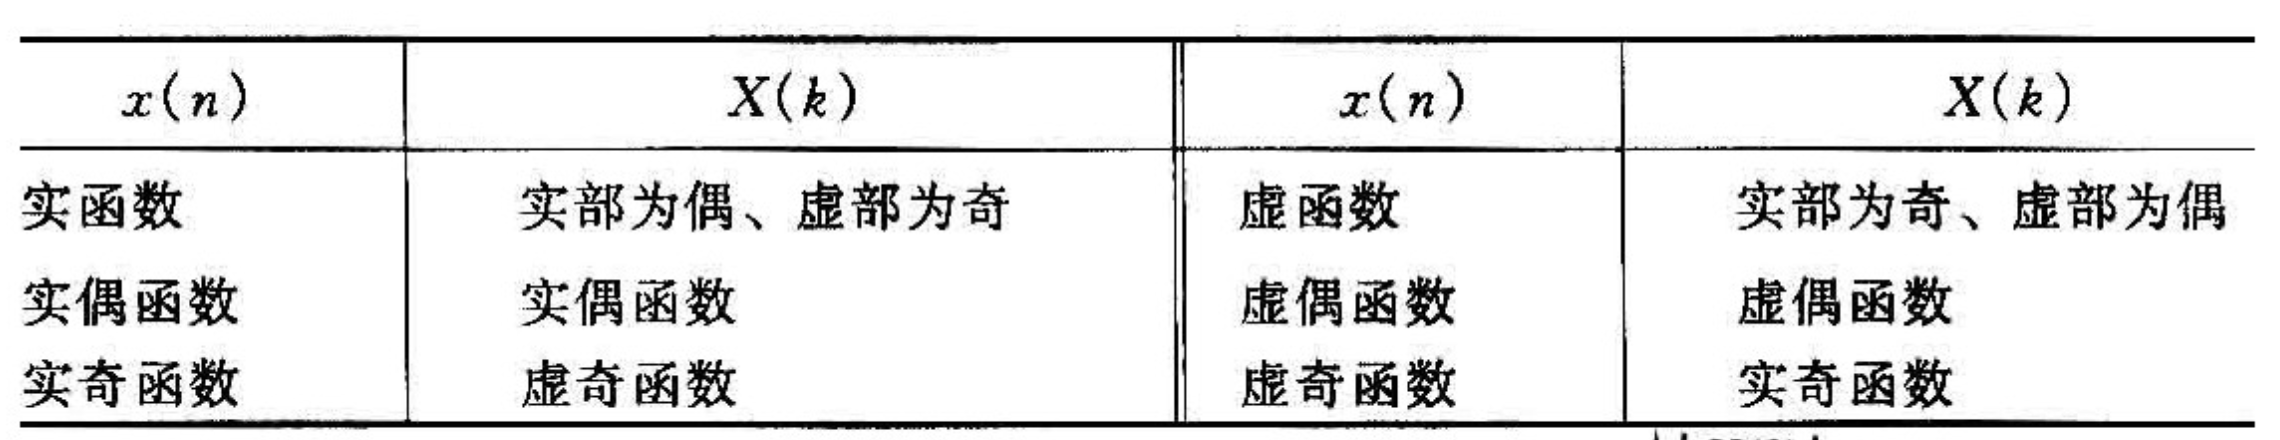
\includegraphics[width=\linewidth]{figure/dft.png}
\end{figure}
\vspace{-10pt}



\subsection{FFT}

DFT:每计算一个 $X[k]$,需要 $N$ 次复数乘法和 $N-1$ 次复数加法;需要算 \(N\) 个。

FFT:
复数乘法:\(\frac{N}{2}\cdot \log_2{N}\)\\
复数加法:\(N\cdot \log_2N\)

\subsection{快速卷积}
线:\(M\times N\); \((M-1)(N-1)\)

FFT:\(L\geq M+N-1\),取\(2^n\)\\
\(3\times\frac{L}{2}\log_2{L}+L\); \(3\times L\log_2{L}\)


\vspace{-10pt}
\begin{figure}[H]
    \centering
    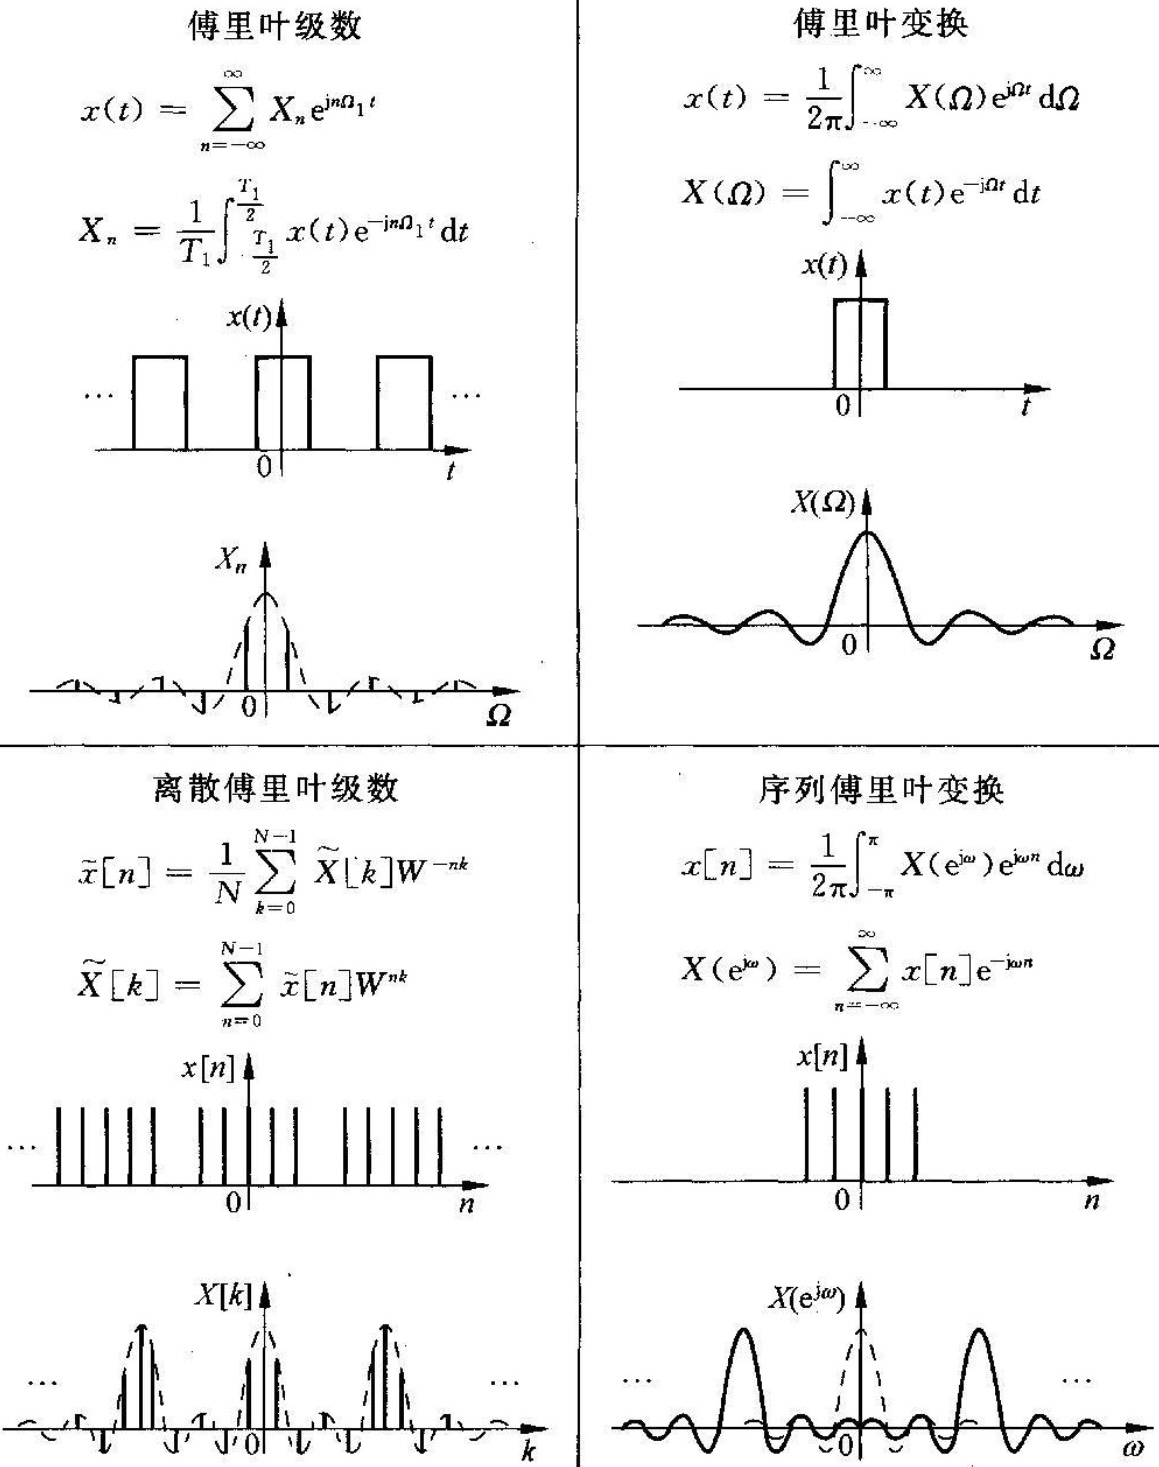
\includegraphics[width=\linewidth]{figure/Pasted image 20220611010632.jpg}
\end{figure}